\documentclass[12pt, paper=a4]{article}
\usepackage[utf8]{inputenc}
\usepackage[german]{babel}
\usepackage{mathrsfs}
\usepackage{amsmath}
\usepackage{amssymb}
\usepackage{listings}
\usepackage{graphicx}
\usepackage{fancyhdr}

\setlength{\parindent}{0pt}

\author{Mareike G\"ottsch, 6695217, Gruppe 2\\Paul H\"olzen, 6673477, Gruppe 1\\Sven Schmidt, 6217064, Gruppe 1}

\title{FGI 2 Hausaufgaben 9}

\rhead{M. G\"ottsch, G-2; P. H\"olzen, G-1; S. Schmidt, G-1}
\pagestyle{fancy}
\begin{document}
\maketitle
\section*{9.3}

\subsection*{1.}

\subsection*{2.}
Als \"Uberdeckungsgraph zu \(N_{9.3}\) f\"ur die Anfangsmarkierung \(m_0=(2,1,0)^t\) ergibt sich:
\begin{figure}[h!]
	\centering
	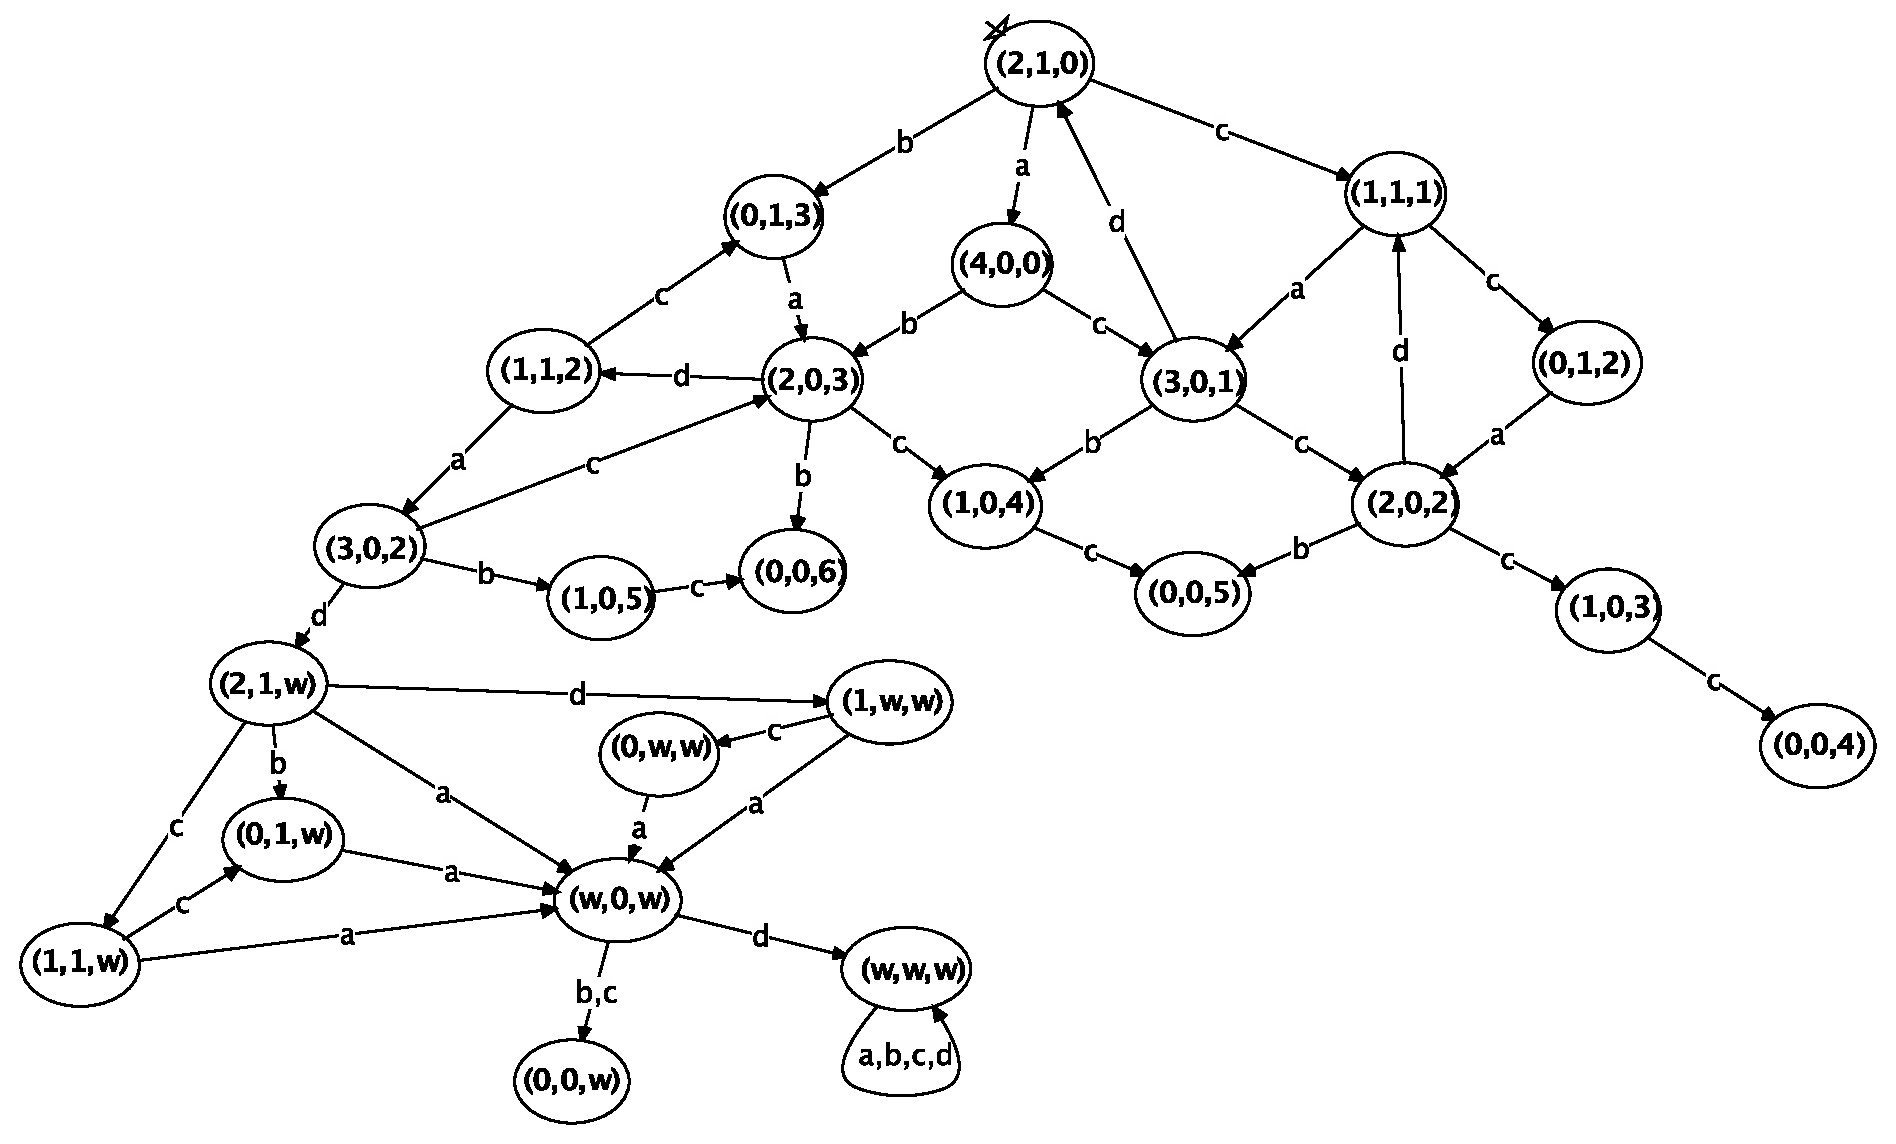
\includegraphics[scale=0.35]{9_3_2.pdf}
	\caption{\"Uberdeckungsgraph von \(N_{9.3}\)}
\end{figure}

\subsection*{3.}


\section*{Aufgabe 9.4}
\subsection*{1.}
\begin{center}
\begin{tabular}{ | c | c c c c c c | c | c | c |}
	\hline
	$\Delta_{N_{LS}}$ & $t_1$ & $t_2$ & $t_3$ & $t_4$ & $t_5$ & $t_6$ & \hspace*{10pt} & $i_1$ & $i_2$\\
	\hline
	$pa$ & -1 & 0 & 1 & -1 & 0 & 1 & & 1 & 0\\
	$pp$ & 0 & -1 & 1 & 0 & -4 & 4 & & 0 & 1\\
	$p_1$ & 1 & -1 & 0 & 0 & 0 & 0 & & 1 & 0\\
	$p_2$ & 0 & 1 & -1 & 0 & 0 & 0 & & 1 & 1\\
	$p_3$ & 0 & 0 & 0 & 1 & -1 & 0 & & 1 & 0\\
	$p_4$ & 0 & 0 & 0 & 0 & 1 & -1 & & 1 & 4\\
	\hline
	& & & & & &\\ \cline{1-7}
	$j_1$ & 1 & 1 & 1 & 1 & 1 & 1\\
	$j_2$ & 0 & 0 & 0 & 1 & 1 & 1\\
	\cline{1-7}
\end{tabular}
\end{center}


P-Invarianten:\\
\begin{align*}
\Delta i_1 &= \Delta_{N_{LS}} \cdot \begin{pmatrix}1 \\ 0 \\ 1 \\ 1 \\ 1 \\ 1\end{pmatrix} = 
\begin{pmatrix}-1+1 \\ -1 \cdot 0-1+1\\ 1+1 \cdot 0-1 \\ -1+1 \\ -4 \cdot 0-1+1 \\ 1+4 \cdot 0-1\end{pmatrix} = 
\begin{pmatrix}0 \\ 0 \\ 0 \\ 0 \\ 0 \\ 0\end{pmatrix}
\\
\Delta i_2 &= \Delta_{N_{LS}} \cdot \begin{pmatrix}0 \\ 1 \\ 0 \\ 1 \\ 0 \\ 4\end{pmatrix} = 
\begin{pmatrix}0 \\ -1+1 \\ 1 \cdot 0+1-1 \\ 0 \\ -4 \cdot 1+-1 \cdot 0+1 \cdot 4 \\ 1 \cdot 0+4 \cdot 1-1 \cdot 4\end{pmatrix} =
\begin{pmatrix}0 \\ 0 \\ 0 \\ 0 \\ 0 \\ 0\end{pmatrix}
\end{align*}

T-Invarianten:\\
\begin{align*}
\Delta j_1 &= \Delta_{N_{LS}} \cdot \begin{pmatrix}1 \\ 1 \\ 1 \\ 1 \\ 1 \\ 1\end{pmatrix} = 
\begin{pmatrix}-1+1-1+1 \\ -1+1-4+4 \\ 1-1 \\ 1-1 \\ 1-1 \\ 1-1\end{pmatrix} = 
\begin{pmatrix}0 \\ 0 \\ 0 \\ 0 \\ 0 \\ 0\end{pmatrix}
\\
\Delta j_2 &= \Delta_{N_{LS}} \cdot \begin{pmatrix}0 \\ 0 \\ 0 \\ 1 \\ 1 \\ 1\end{pmatrix} = 
\begin{pmatrix}-1+1 \\ -4+4 \\ 0 \\ 0 \\ 1-1 \\ 1-1\end{pmatrix} = 
\begin{pmatrix}0 \\ 0 \\ 0 \\ 0 \\ 0 \\ 0\end{pmatrix}
\end{align*}

\subsection*{2.}
\begin{center}
\begin{tabular}{ | c | c c c c c c |}
	\hline
	$\Delta_{N_{Drohne}}$ & $t_1$ & $t_2$ & $t_3$ & $t_4$ & $t_5$ & $t_6$\\
	\hline
	$p_1$ & -1 & 0 & 0 & 0 & 0 & 1\\
	$p_2$ & 1 & -1 & 0 & 0 & 0 & 0\\
	$p_3$ & 0 & 1 & -1 & 0 & 0 & 0\\
	$p_4$ & 0 & 0 & 1 & -1 & 0 & 0\\
	$p_5$ & -1 & 0 & 0 & 0 & 0 & 1\\
	$p_6$ & 0 & -1 & 0 & 0 & 1 & 0\\
	$p_7$ & 0 & 0 & 0 & 1 & -1 & 0\\
	$p_8$ & 0 & 0 & 0 & 0 & 1 & -1\\
	\hline	
\end{tabular}
\end{center}


\subsection*{3.}
Die Menge aller S-Invariantenvektoren ist die Menge der Vektoren $i^{tr} = (i_0 ... i_7)$, die das folgende Gleichungssystem lösen:\\

\begin{align*}
&I) &-i_0 + i_1 - i_4 &= 0\\
&II) &-i_1 + i_2 - i_5 &= 0\\
&III) &-i_2 + i_3 &= 0\\
&IV) &-i_3 + i_6 &= 0\\
&V) &i_5 - i_6 + i_7 &= 0\\
&VI) &i_0 + i_4 - i_7 &= 0\\
\end{align*}

\subsection*{5.}
\begin{center}
\begin{tabular}{ | c | c c c c c c c |}
	\hline
	$\Delta_{N_{Drohne}}$ & $t_1$ & $t_2$ & $t_3$ & $t_4$ & $t_5$ & $t_6$ & $t_7$\\
	\hline
	$p_1$ & -1 & 0 & 0 & 0 & 0 & 1 & 0\\
	$p_2$ & 1 & -1 & 0 & 0 & 0 & 0 & 0\\
	$p_3$ & 0 & 1 & -1 & 0 & 0 & 0 & 0\\
	$p_4$ & 0 & 0 & 1 & -1 & 0 & 0 & 0\\
	$p_5$ & -1 & 0 & 0 & 0 & 0 & 0 & 1\\
	$p_6$ & 0 & -1 & 0 & 0 & 1 & 0 & 0\\
	$p_7$ & 0 & 0 & 0 & 1 & -1 & 0 & 0\\
	\hline	
\end{tabular}
\end{center}

\section*{Aufgabe 9.5}
	\begin{itemize}
	\item In einem Workflow-Netz sind Quelle a und Senke e beliebig zu w\"ahlen.\\
		Wahr oder falsch?\\
		\textit{(Lesestoff Woche 9, Teil 1)}
	\item Eine Transition kann sowohl einen Uplink als auch (mehrere) Downlinks haben.\\
		Wahr oder falsch?\\
		\textit{(Lesestoff Woche 9, Teil 2)}
	\end{itemize}
\end{document}
